
% This LaTeX was auto-generated from an M-file by MATLAB.
% To make changes, update the M-file and republish this document.

\documentclass{article}
\usepackage{graphicx}
\usepackage{color}

\sloppy
\definecolor{lightgray}{gray}{0.5}
\setlength{\parindent}{10pt}
\usepackage[margin=1in]{geometry}

\begin{document}

\title{Dynamical Adaptation in ORNs}
\author{Srinivas Gorur-Shandilya}
\maketitle

    
    
\subsection*{Contents}

\begin{itemize}
\setlength{\itemsep}{-1ex}
   \item Stimulus Characteristics
   \item Stimulus and Response Statistics
   \item Variable Response
   \item DA Model fit to Data
\end{itemize}
\begin{par}
How do ORNs respond to non-Gaussian inputs? Real odor stimuli are characterised by long tails and non-gaussian statisitcs, with large whiffs of odor that occur in periods of relatively low signal. Such a stimulus has been generated here, and the responses of ORNs to these signals is analysed in this figure.
\end{par} \vspace{1em}


\subsection*{Stimulus Characteristics}

\begin{par}
The following figure shows what the stimulus and the neuron's looks like.
\end{par} \vspace{1em}

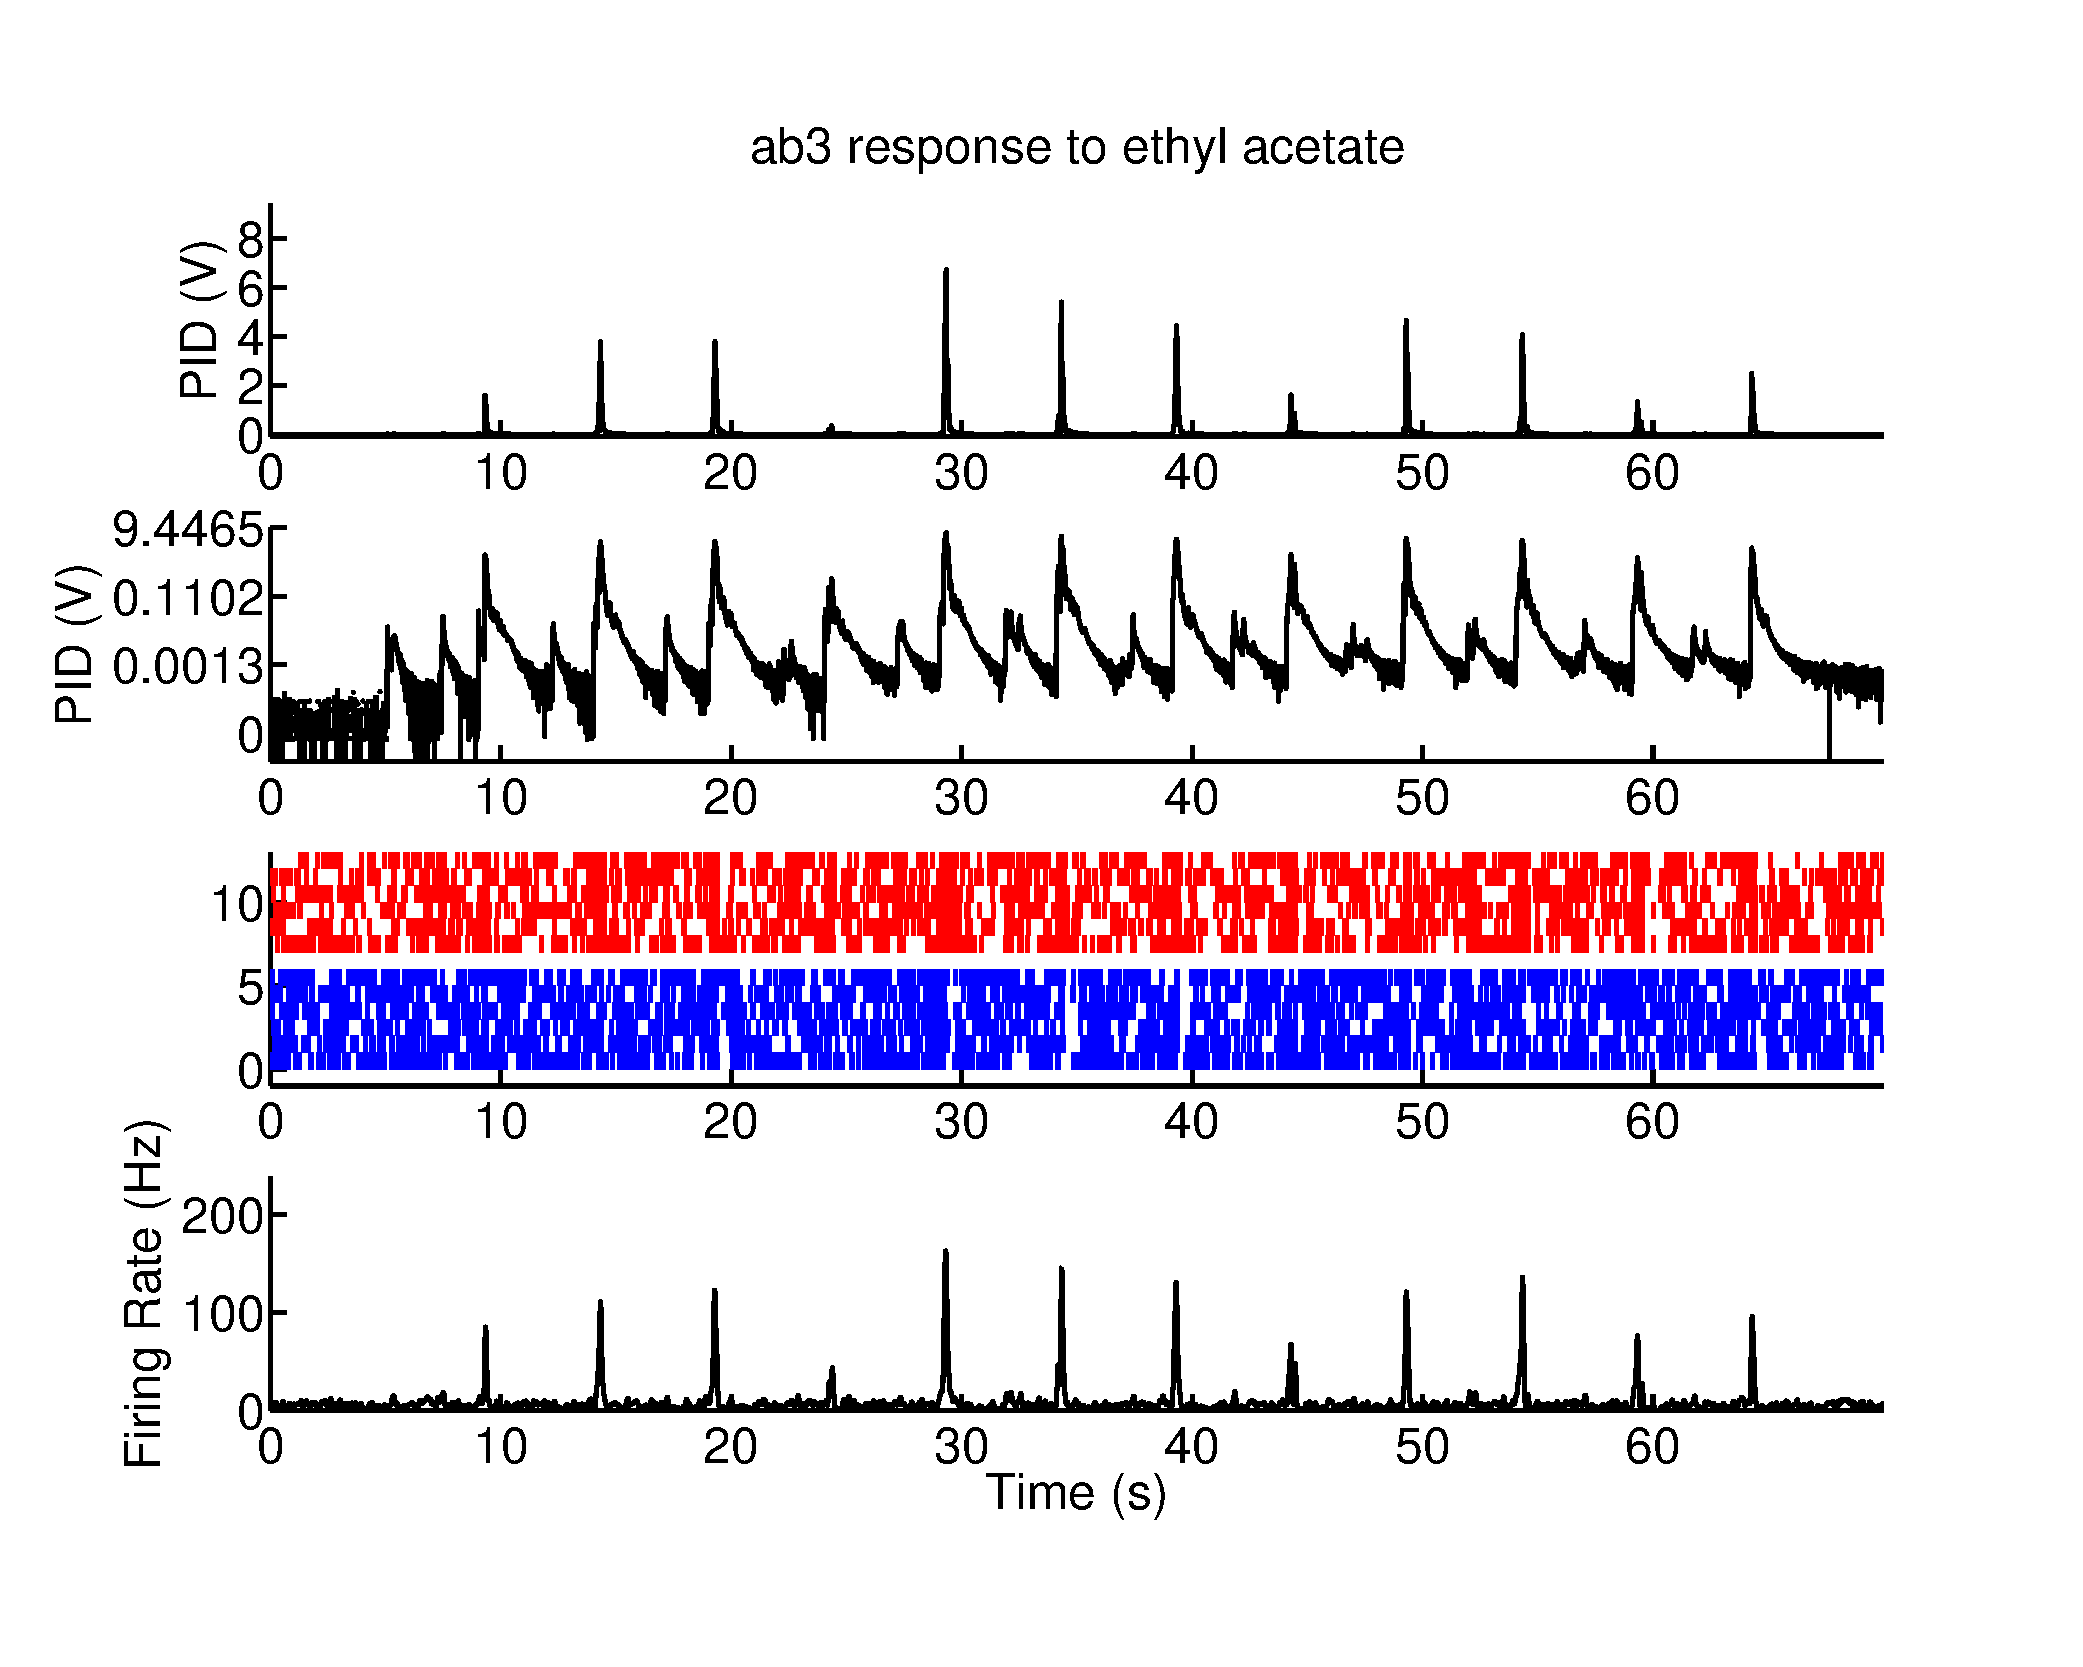
\includegraphics [width=\textwidth]{Mahmut_Data_Analysis_01.pdf}


\subsection*{Stimulus and Response Statistics}

\begin{par}
The following figure describes the statistics of the stimulus and the response. Left panel: Histograms of stimulus and response. Middle panel: Autocorrelation functions of the stimulus and the response. Right: Linear filter extracted from this dataset.
\end{par} \vspace{1em}

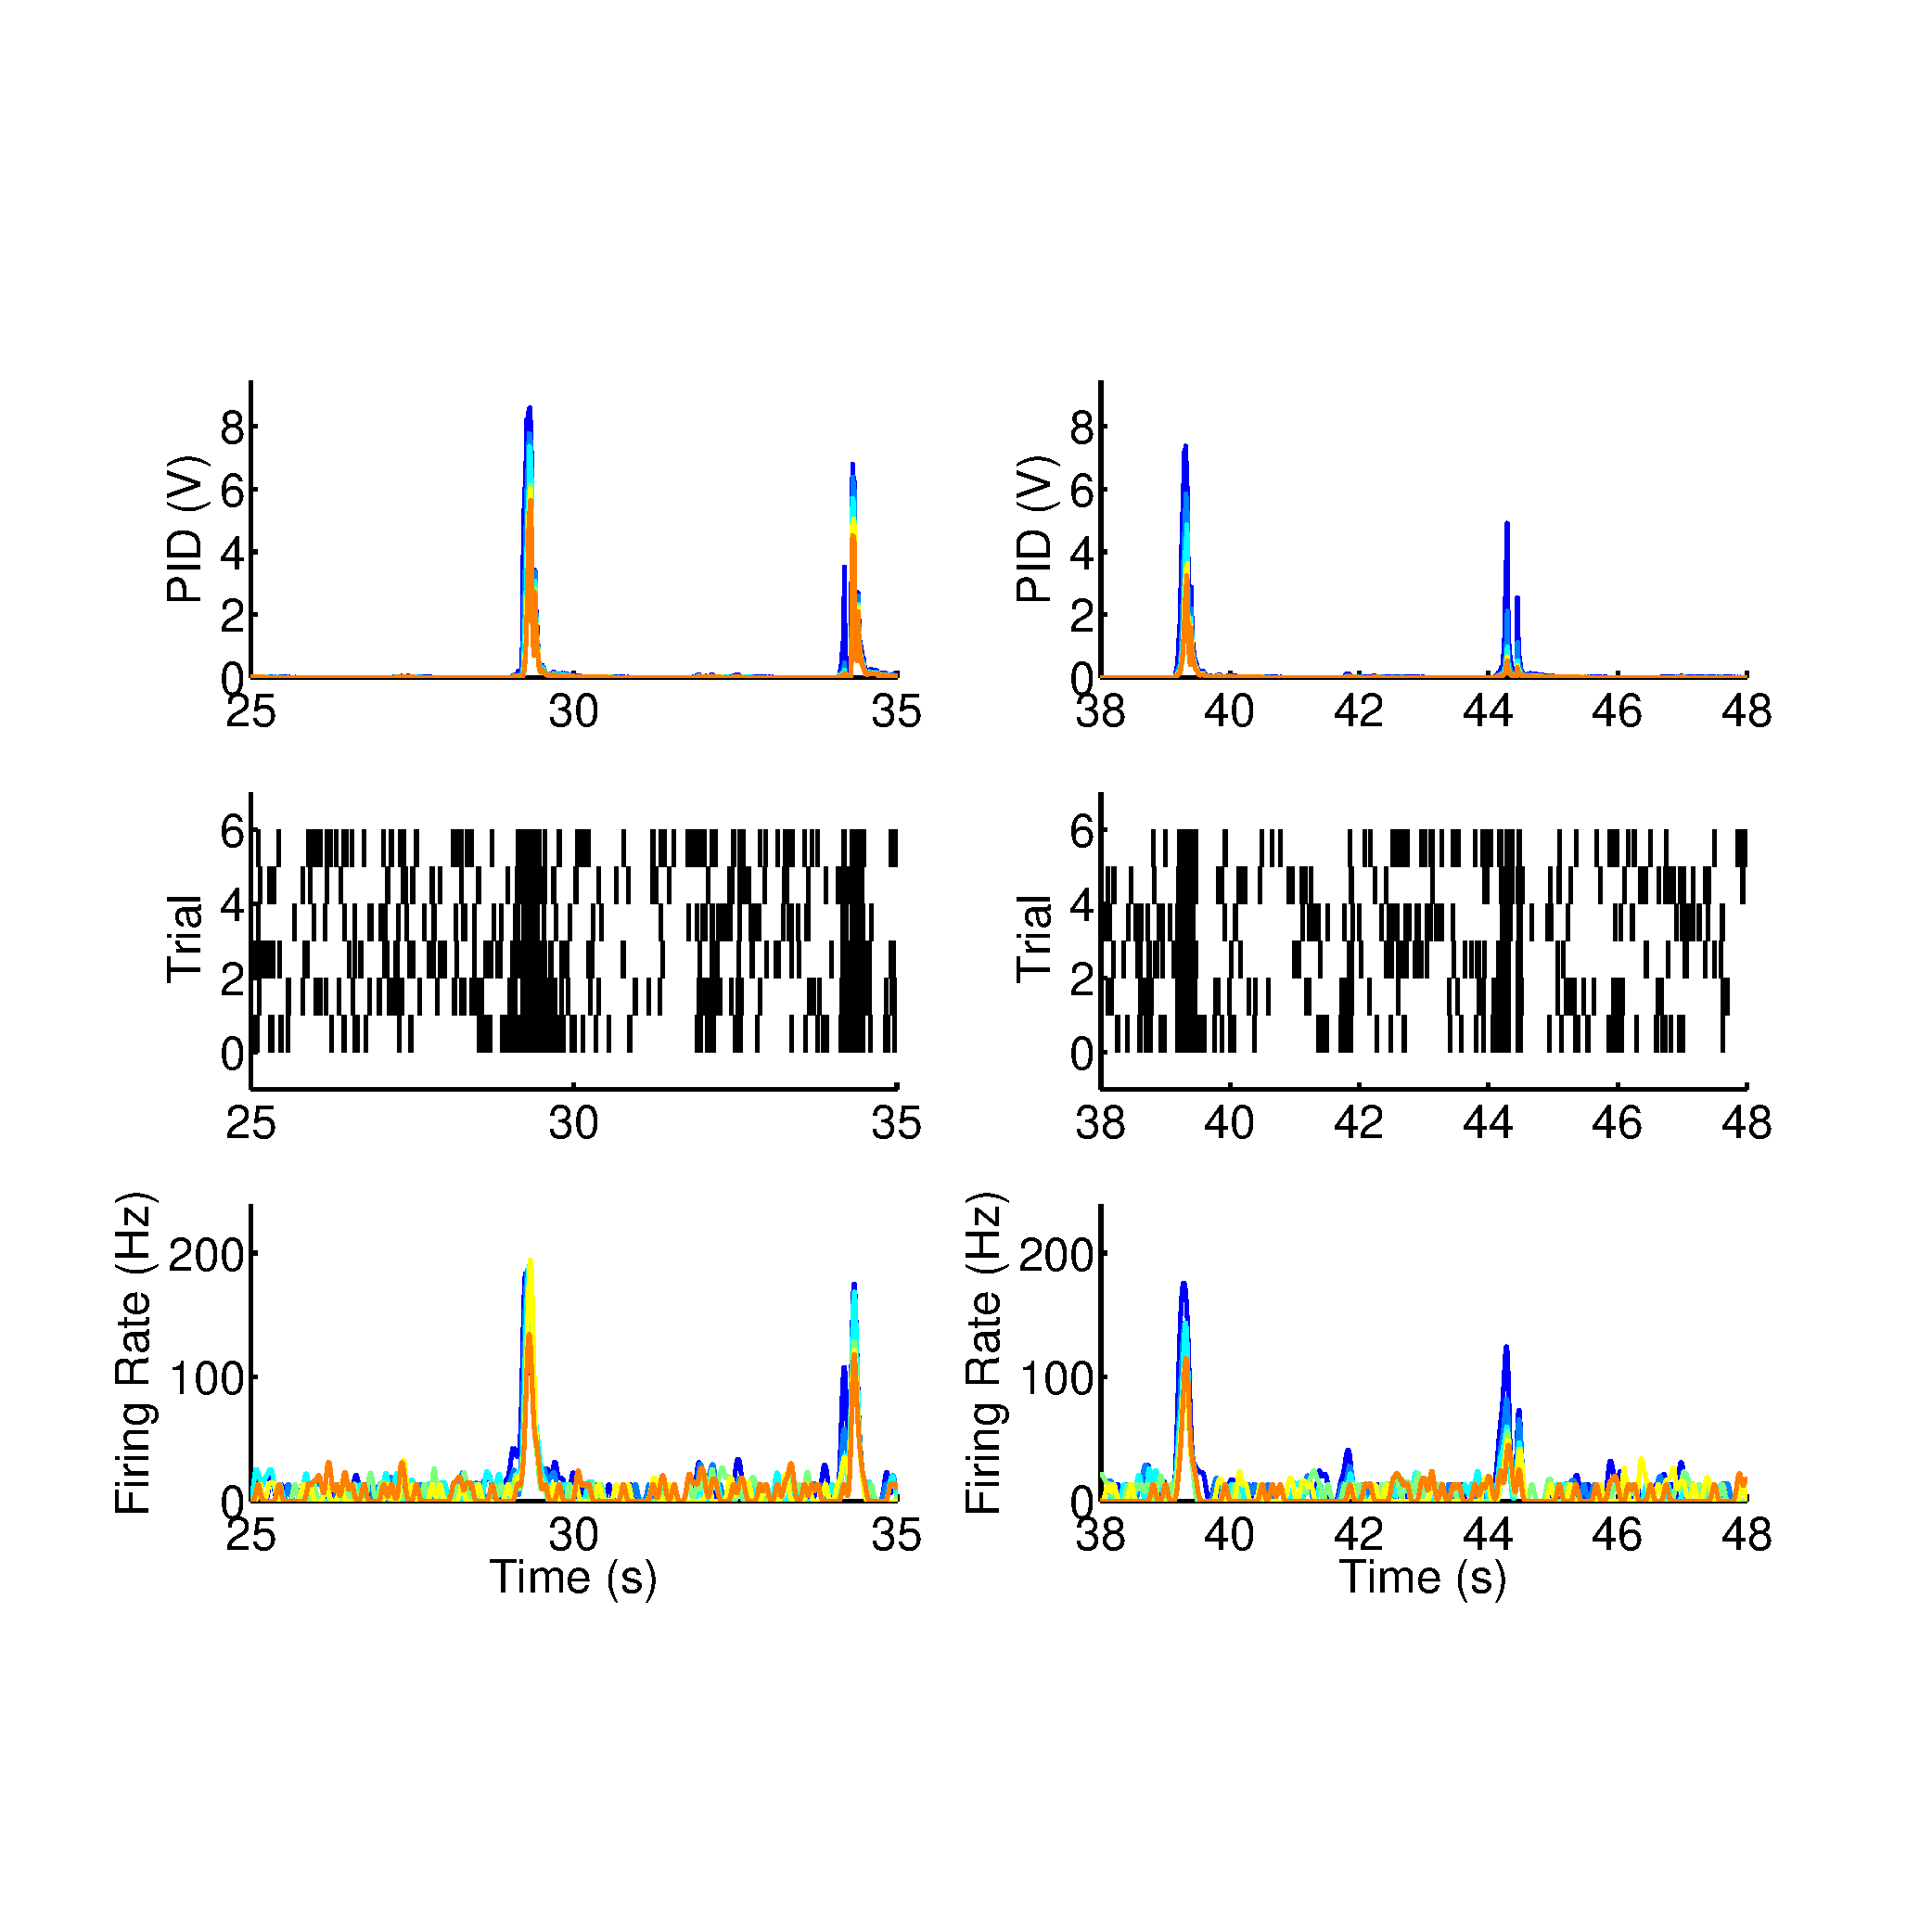
\includegraphics [width=\textwidth]{Mahmut_Data_Analysis_02.pdf}


\subsection*{Variable Response}

\begin{par}
The most intereesting thing about this dataset is that sometimes, for some whiffs, the ORN responds, but for others, it does not. The following figure shows a close-up of the data to illustrate this point. On the left, the traces show that ORNs respond only to some pulses, but not to others. It's not clear why. On the right, the plots show that ORN response to two almost identical pulses is very different, with the response to the second pulse much smaller than the response to the first.
\end{par} \vspace{1em}

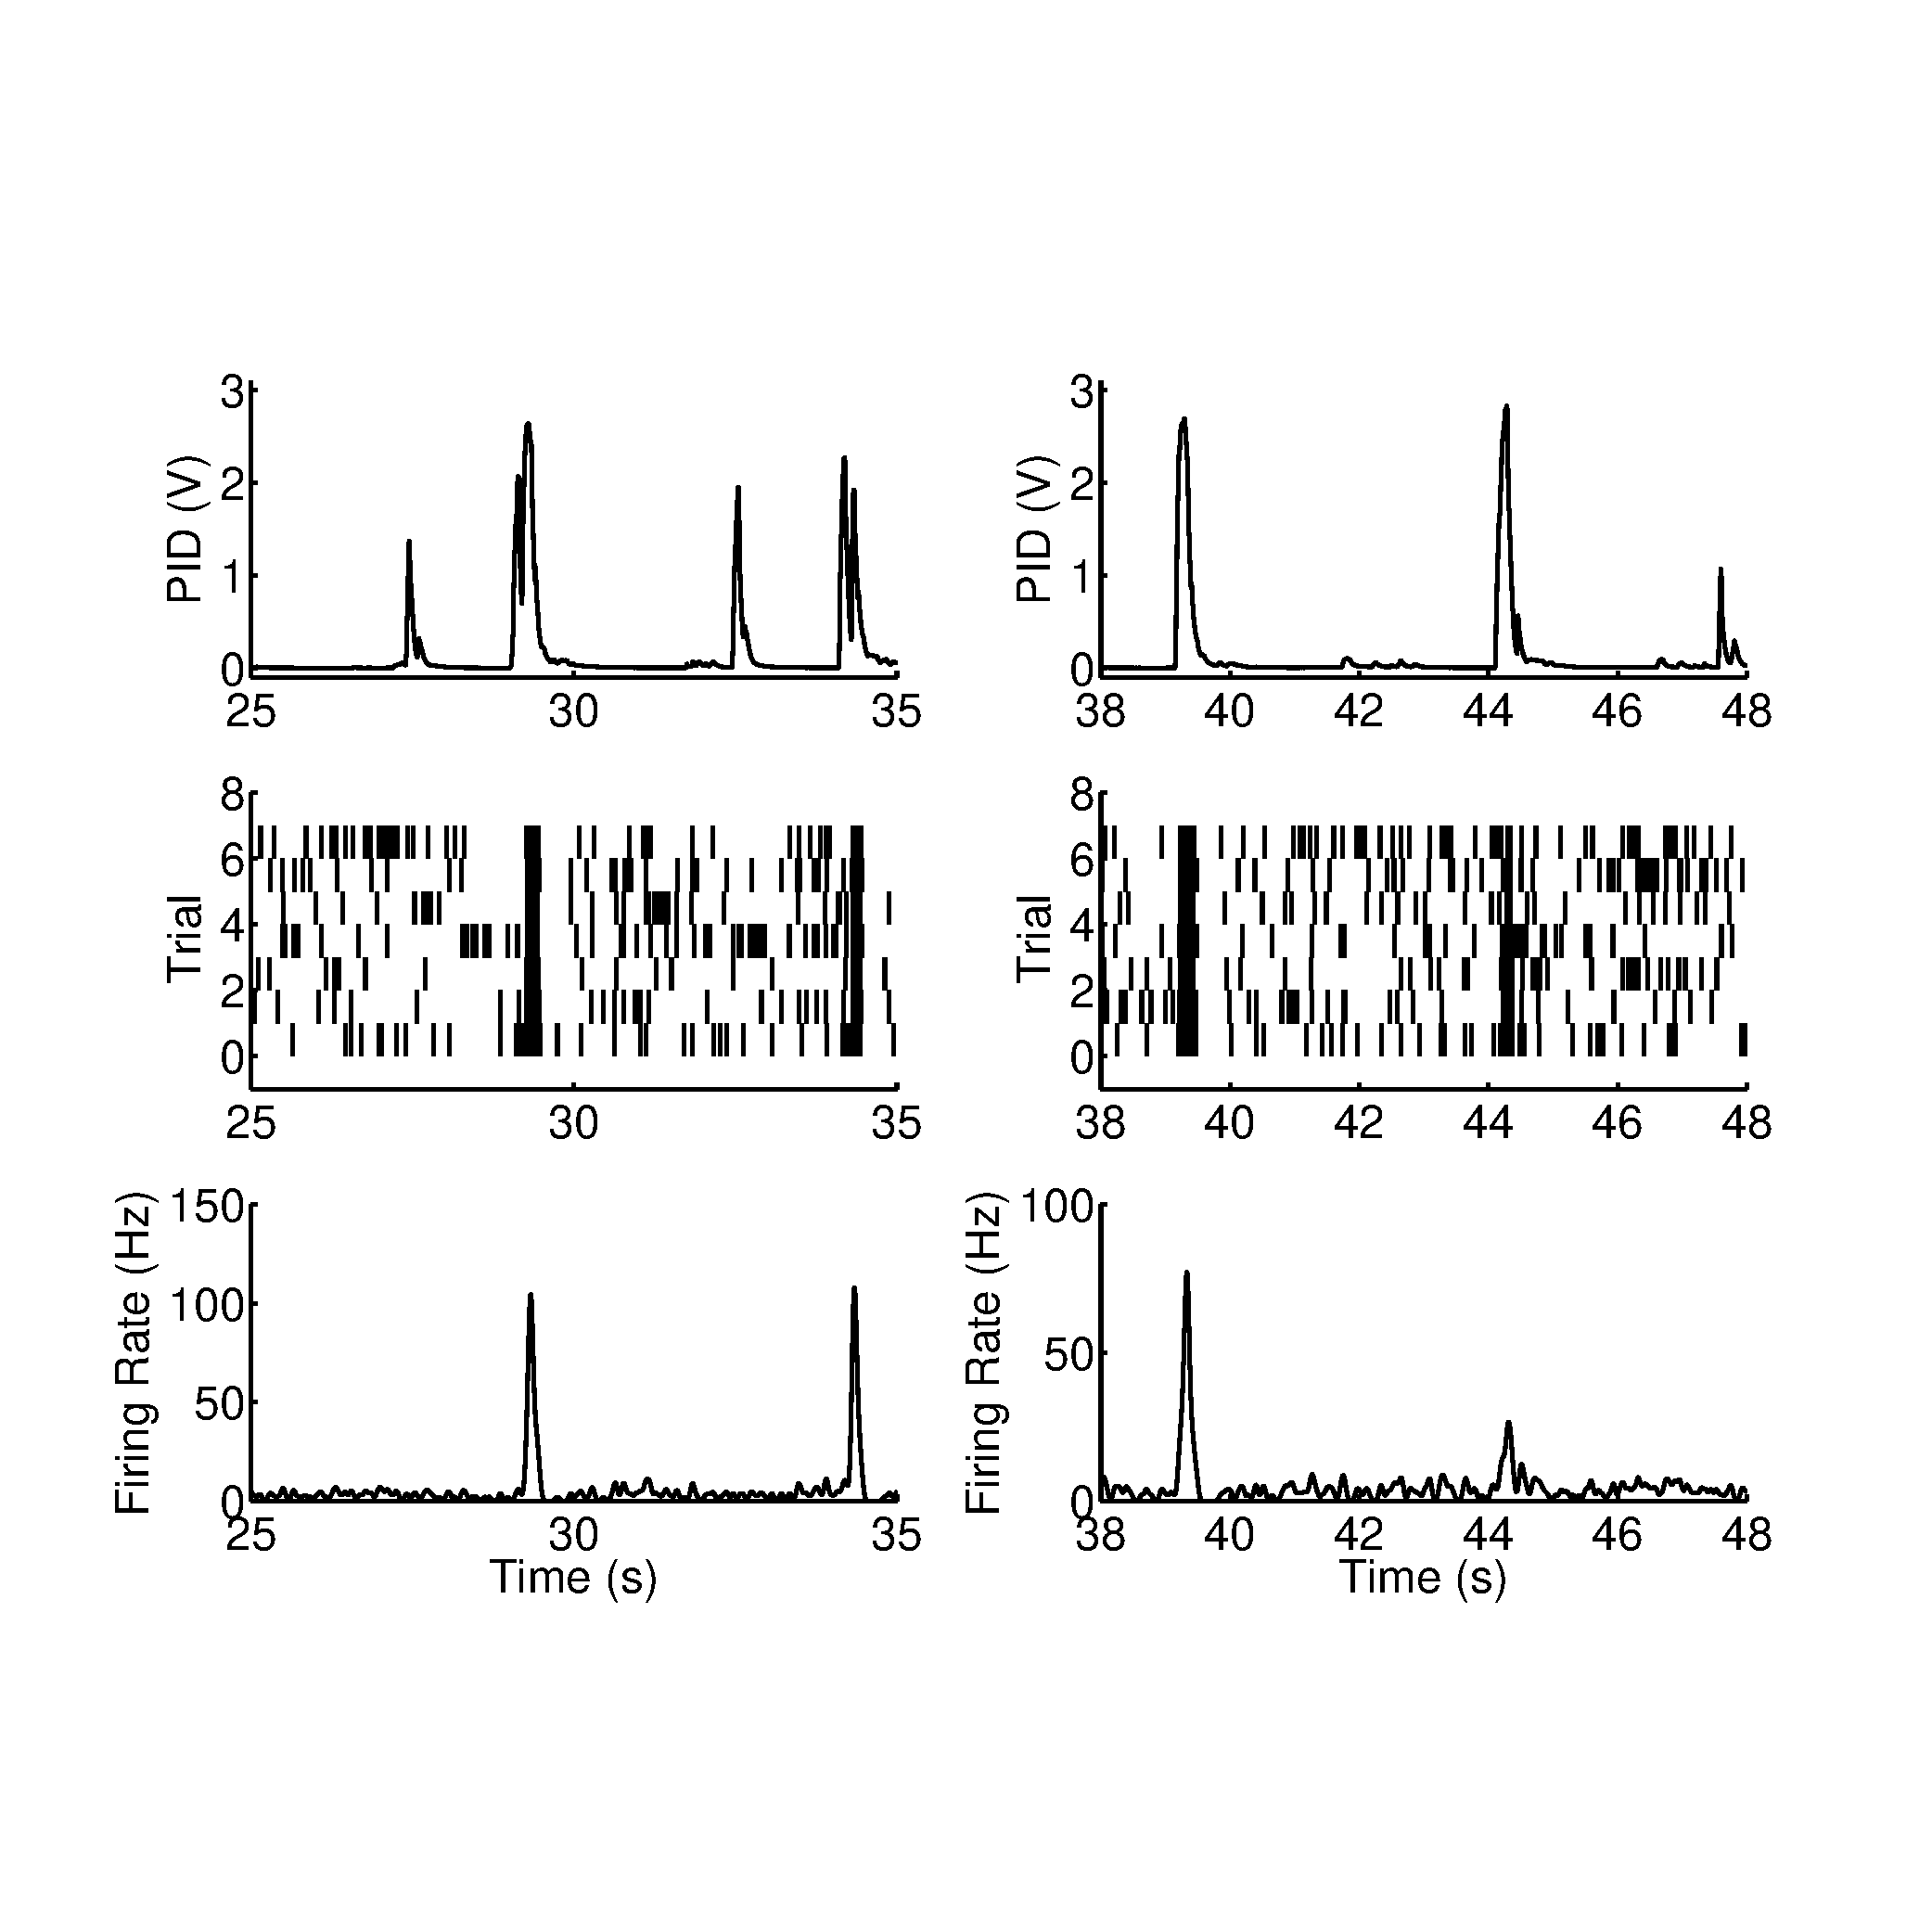
\includegraphics [width=\textwidth]{Mahmut_Data_Analysis_03.pdf}
\begin{par}
Why is there so much variability in the response? The following figure shows a scatter plot of the stimulus and the response.
\end{par} \vspace{1em}

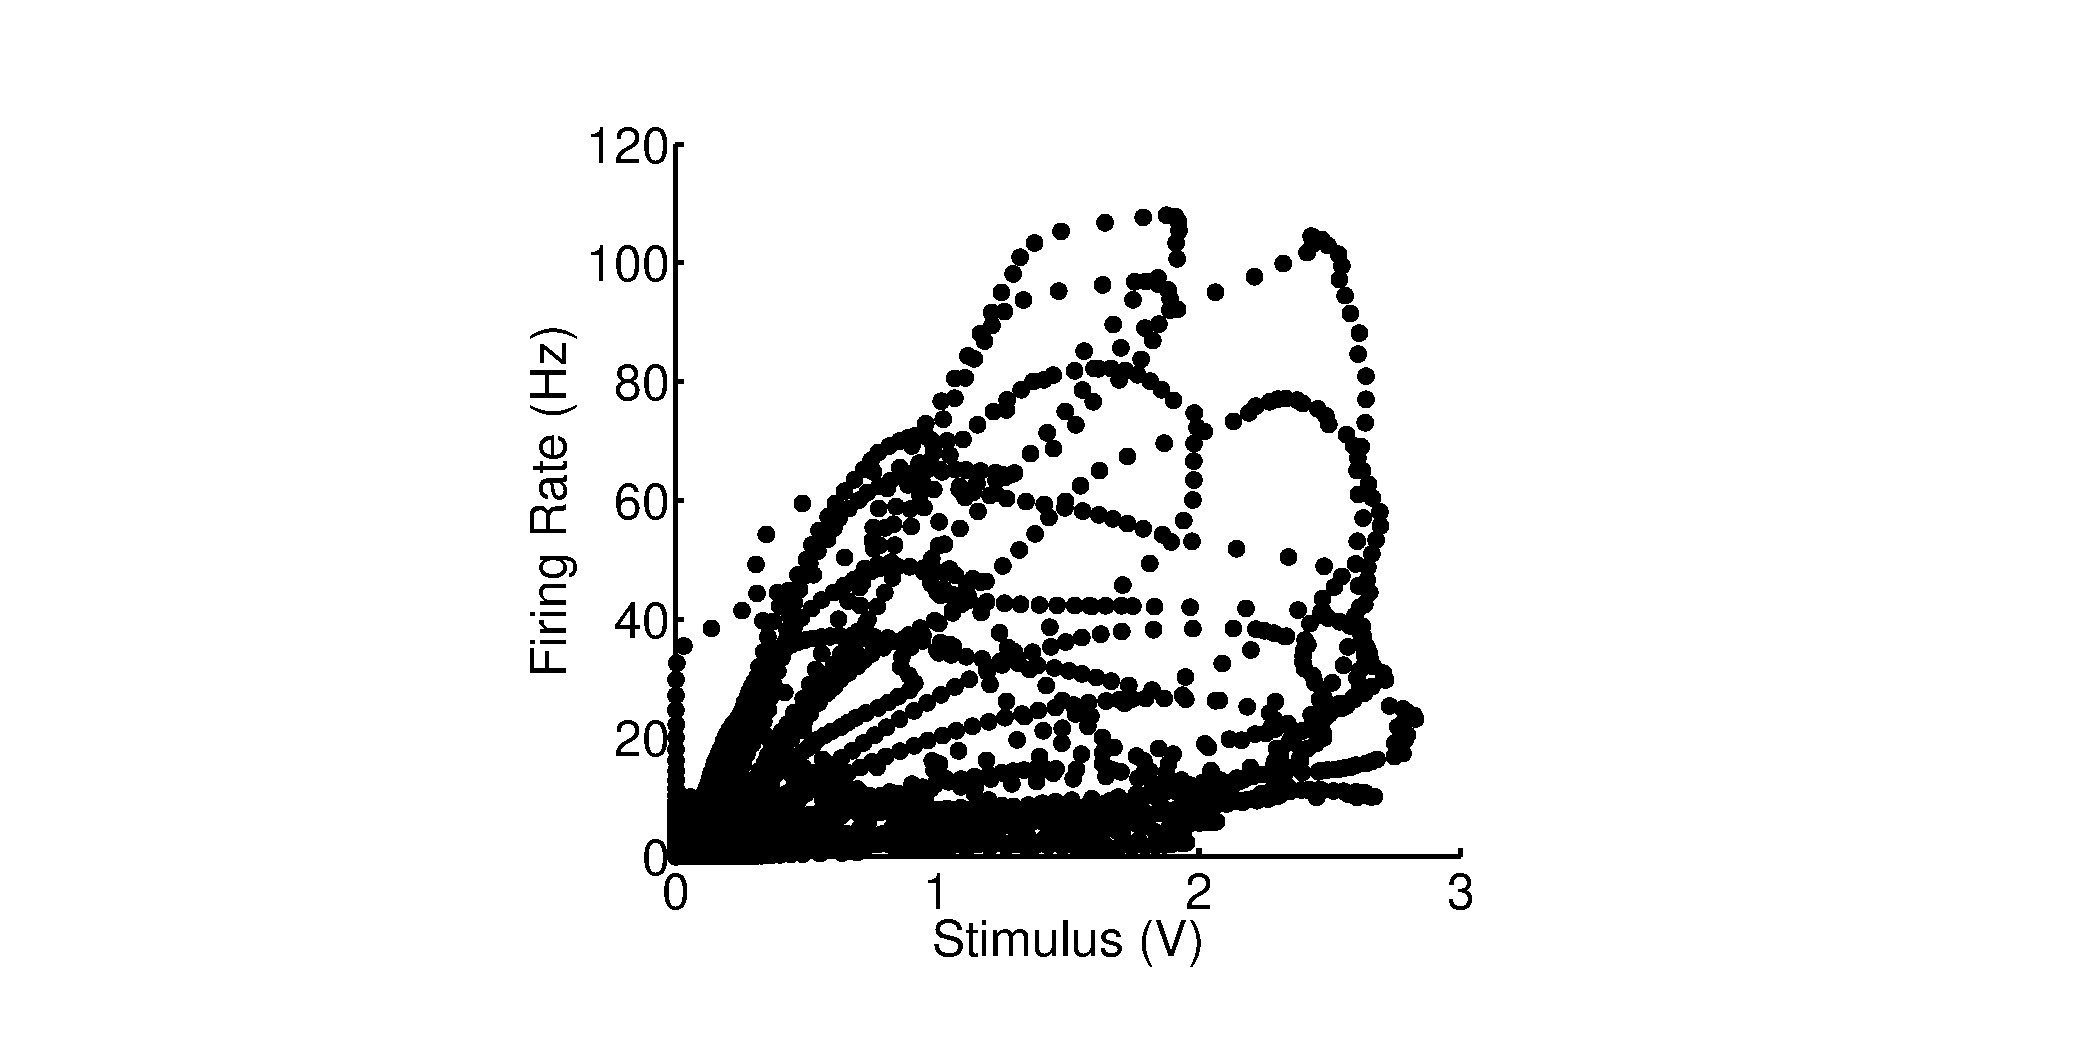
\includegraphics [width=\textwidth]{Mahmut_Data_Analysis_04.pdf}
\begin{par}
There is surprisingly little correlation between the input and the output. In particular, trajectories seem to cover all the space, instead of being confined to one curve. The r-square between the stimulus and the response is:
\end{par} \vspace{1em}

        \color{lightgray} \begin{verbatim}    0.3994

\end{verbatim} \color{black}
    \begin{par}
Let's attempt to find all the times when the stimulus is high, i.e., ten standard deviations above the baseline. This threshold ensures that we pick up all the whiffs, but ignore the blanks in between, as shown in the figure below.
\end{par} \vspace{1em}

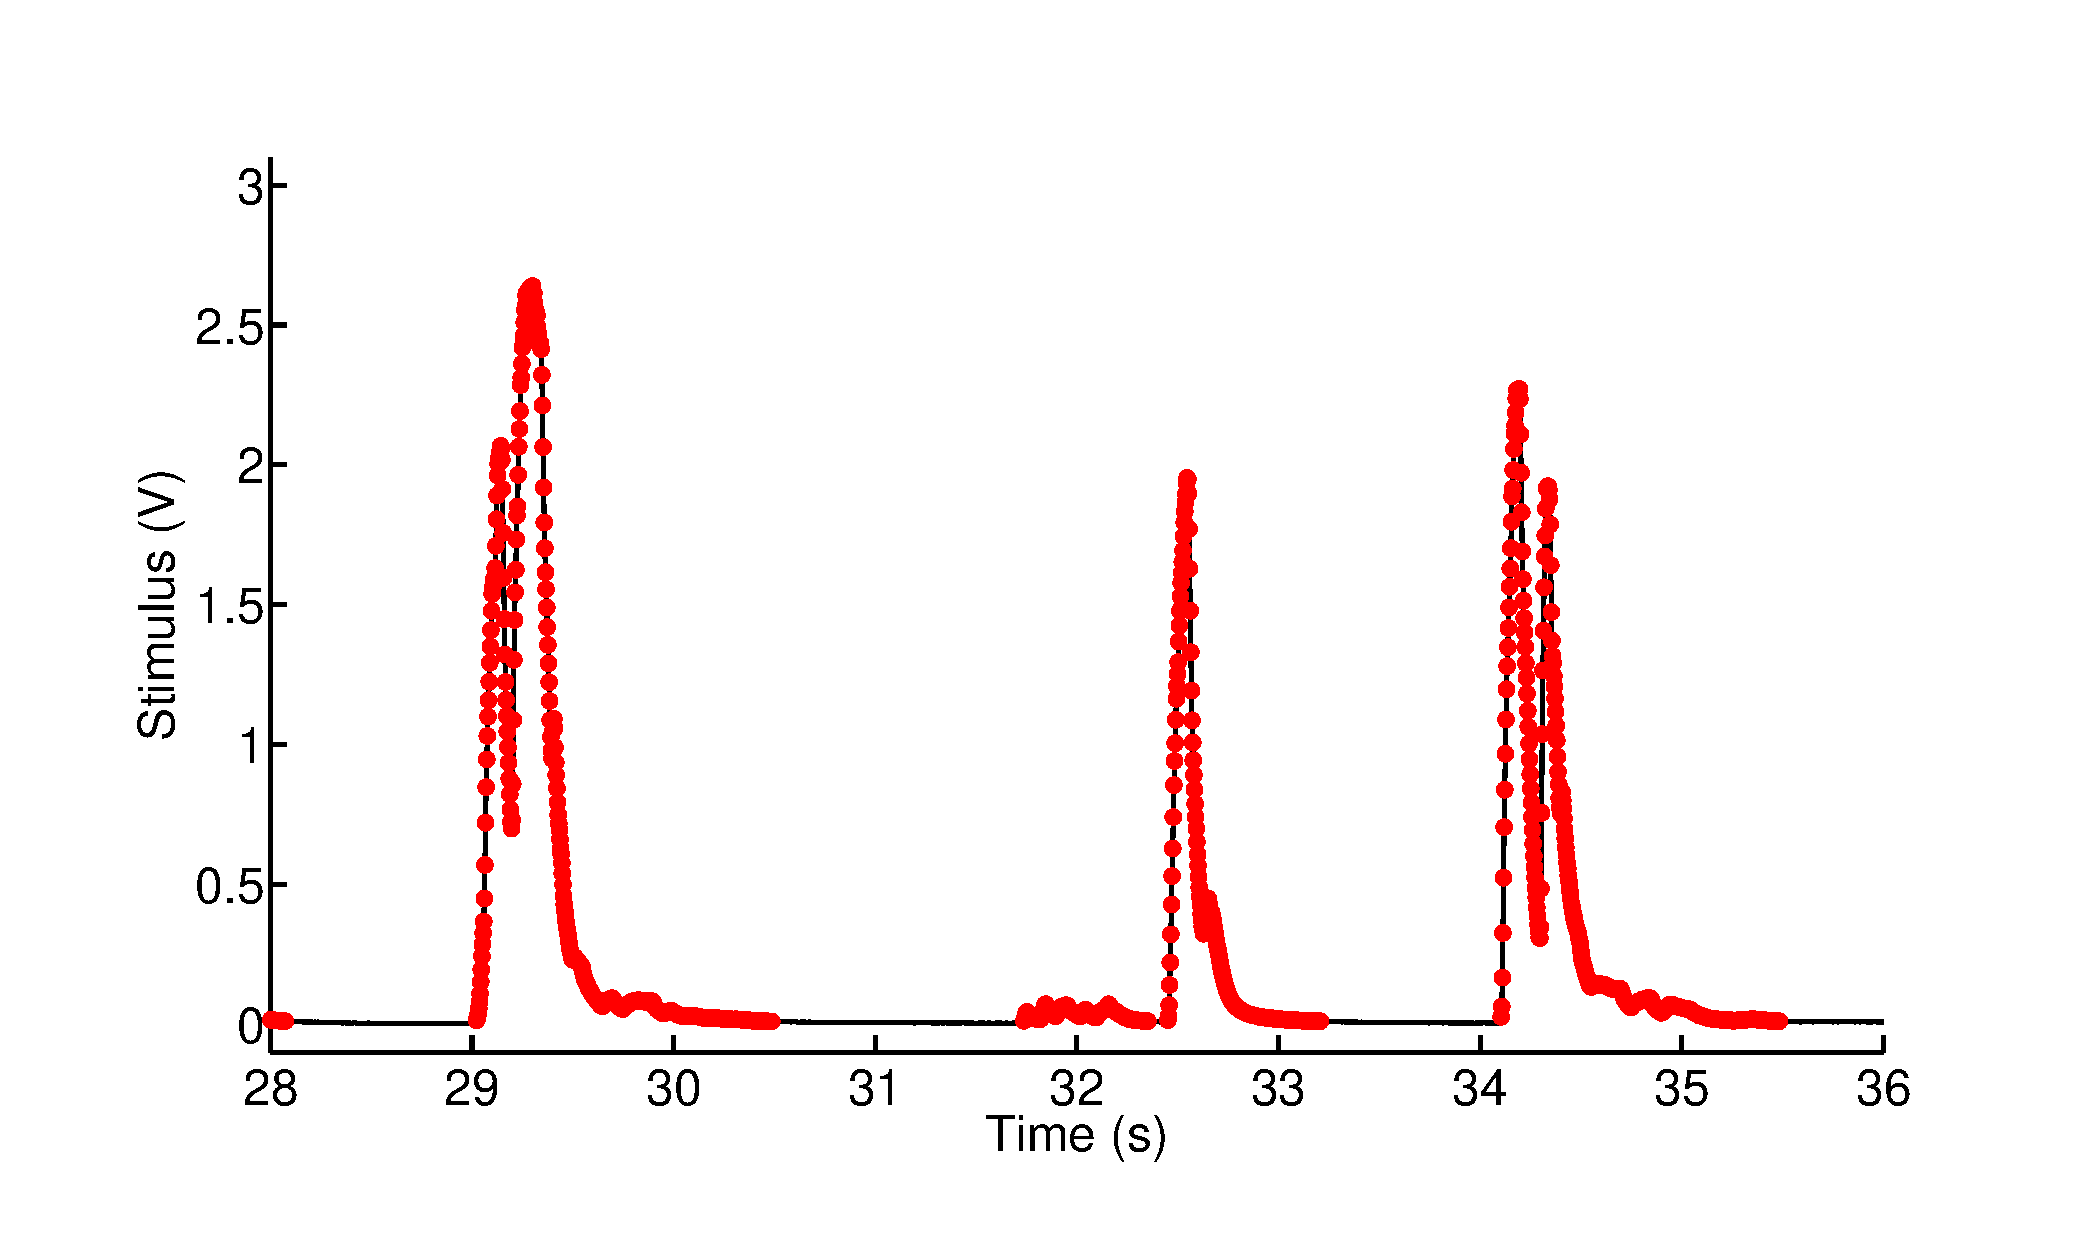
\includegraphics [width=\textwidth]{Mahmut_Data_Analysis_05.pdf}
\begin{par}
Now we break up the trace so that we can perform a whiff-by-whiff analysis of the response. The following figure shows the relationship between response and stimulus on a whiff-by-whiff basis.
\end{par} \vspace{1em}

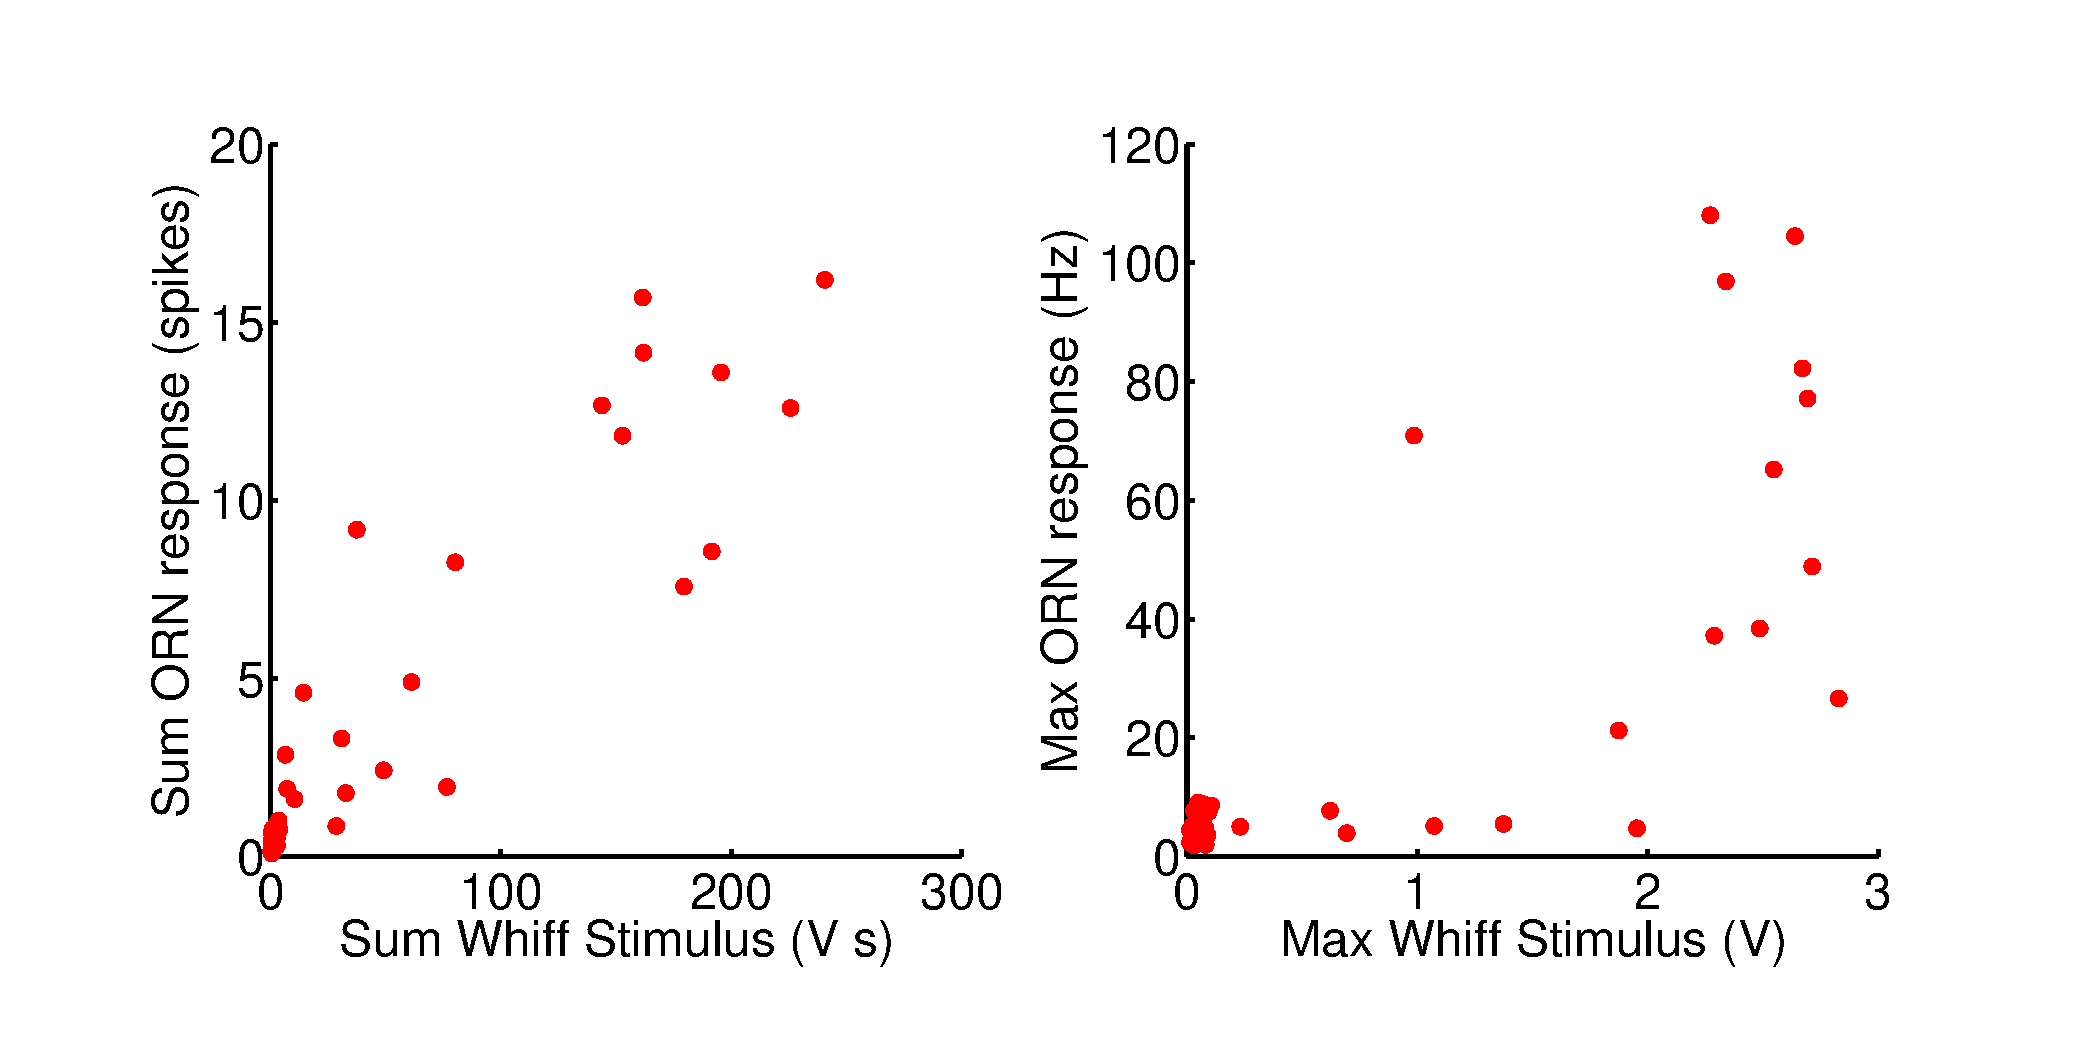
\includegraphics [width=\textwidth]{Mahmut_Data_Analysis_06.pdf}
\begin{par}
The sum total of the odor delivered/whiff seems to correlate well with the number of spikes elicited in that whiff. The r-square of this is:
\end{par} \vspace{1em}

        \color{lightgray} \begin{verbatim}    0.8349

\end{verbatim} \color{black}
    \begin{par}
The examination of the raw data strongly suggests that the response of the ORN seems to depend on the previous stimulus. (e.g., response to pulse at $t=44s$ is half that of a very similar pulse at $t=39s$)
\end{par} \vspace{1em}


\subsection*{DA Model fit to Data}

\begin{par}
Can we fit a DA Model to this data? Does it explain the observed variability? The following figure shows the ORN firing rates and the best-fit DA Model.
\end{par} \vspace{1em}

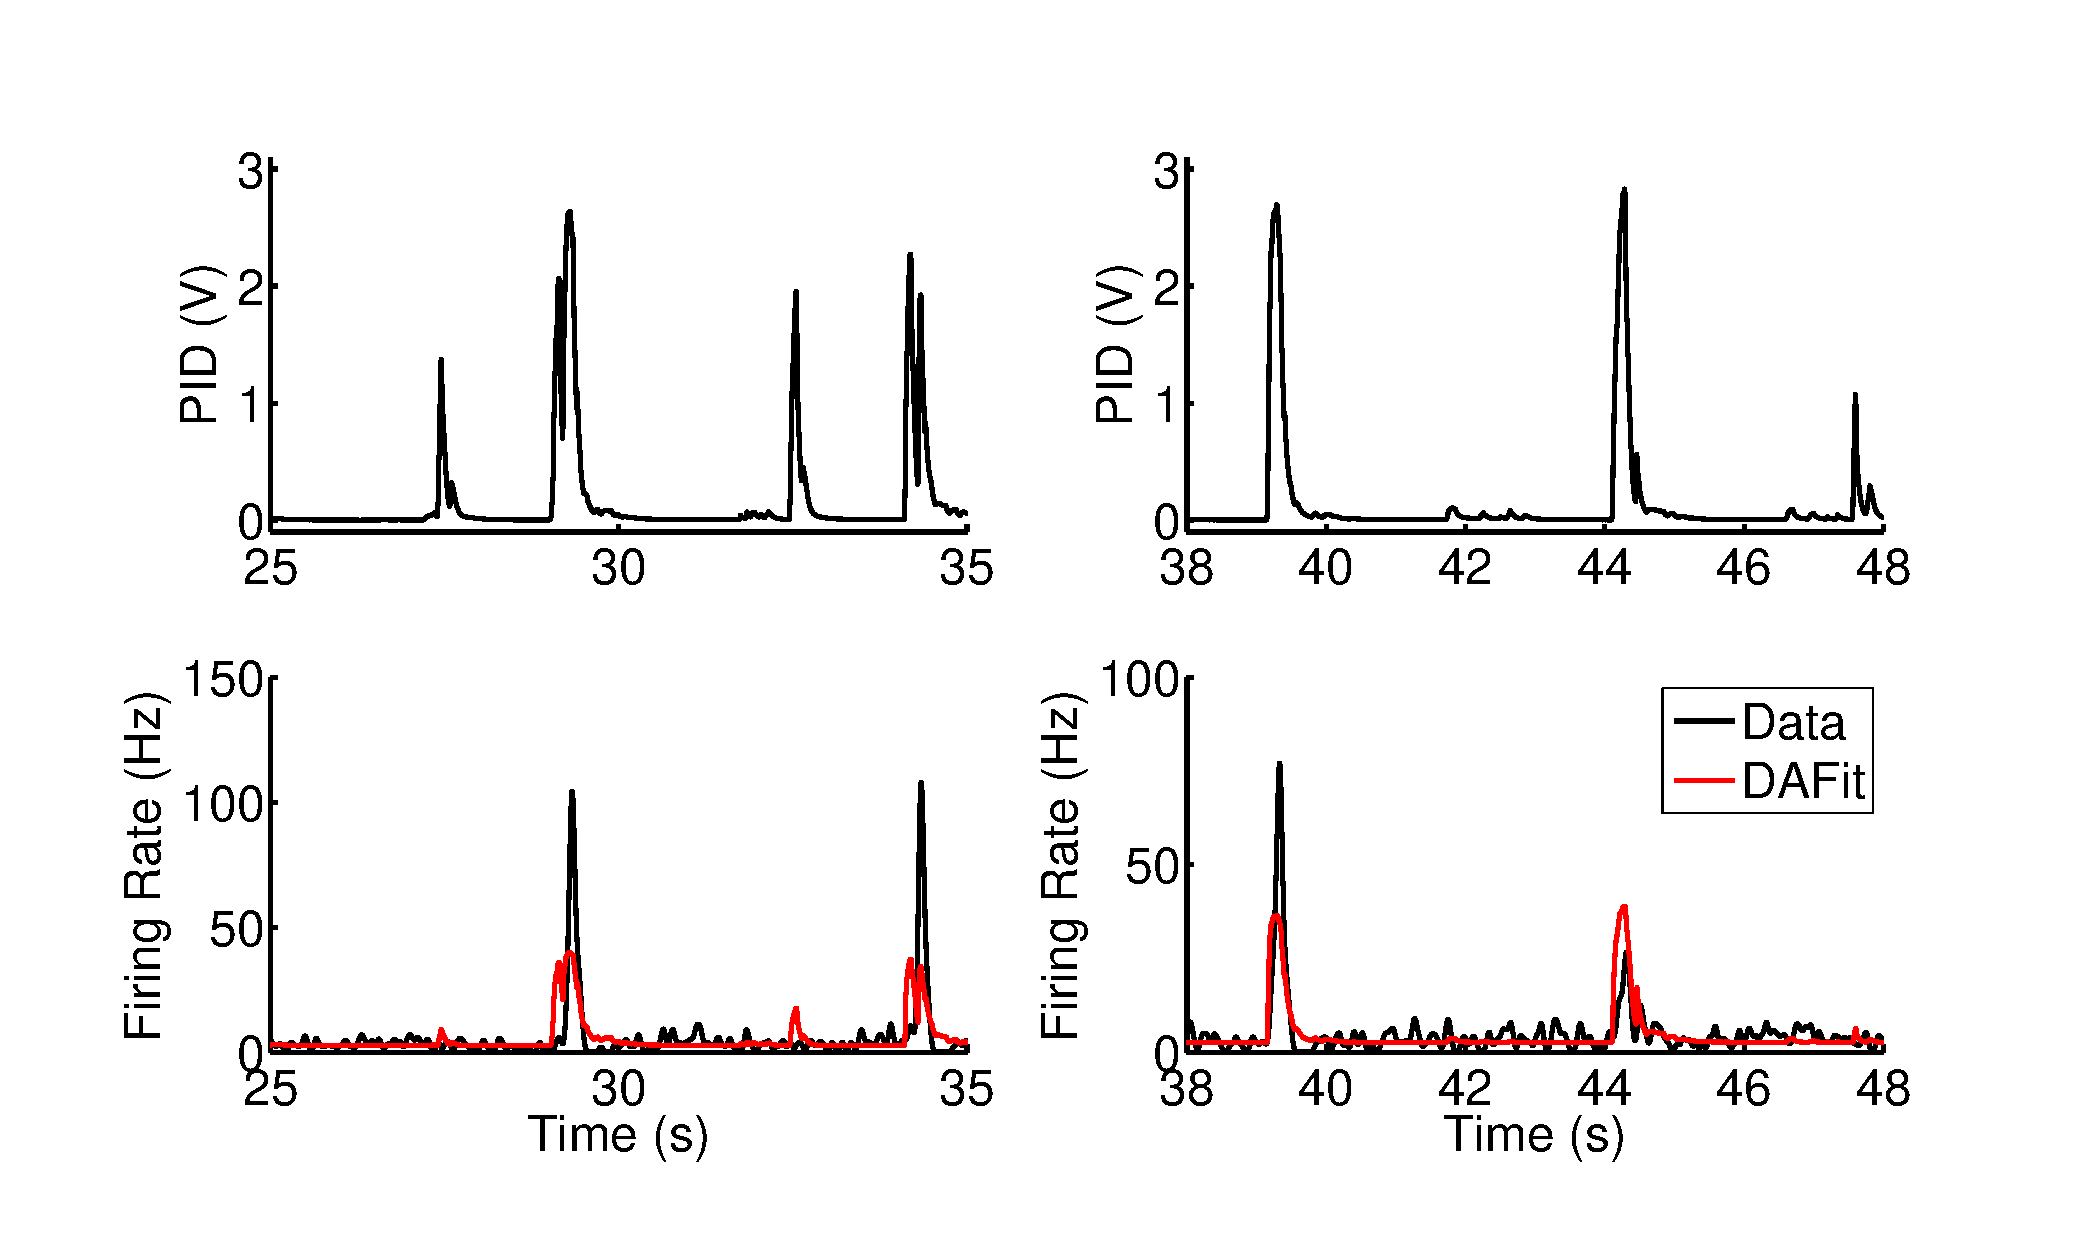
\includegraphics [width=\textwidth]{Mahmut_Data_Analysis_07.pdf}
\begin{par}
The r-square of the fit is:
\end{par} \vspace{1em}

        \color{lightgray} \begin{verbatim}    0.4704

\end{verbatim} \color{black}
    


\end{document}
    
